\section{Half-Edge-Mesh}
Um die oben genannten Problemstellungen zu l\"osen, gibt es andere Ans\"atze Polygonalnetze zu realisieren. Einer dieser L\"osungen ist das Konzept der Half-Edge-Meshes. Ein solches Mesh besteht aus folgenden Komponenten: 
\begin{itemize}
	\item eine Liste von Vertices
	\item eine Liste von Half-Edges
	\item eine Liste von Faces.
\end{itemize}
Der Ansatz des Half-Edge-Mesh sieht dabei vor, dass jede Kante des Netzes aus zwei Half-Edges besteht, sodass jeweils eine Half-Edge auf einen Vertex der Kante zeigt, wie in Abbildung \ref{fig:half-edge-mesh} gezeigt.
Jede Half-Edge besitzt eine Referenz auf die ihr gegen\"uberliegende Half-Edge und auf die ihr Nachfolgende. Zudem referenziert sie die anliegende Face und den Vertex, aus dem sie hervorgeht.
\begin{figure}[t]
	\centering
	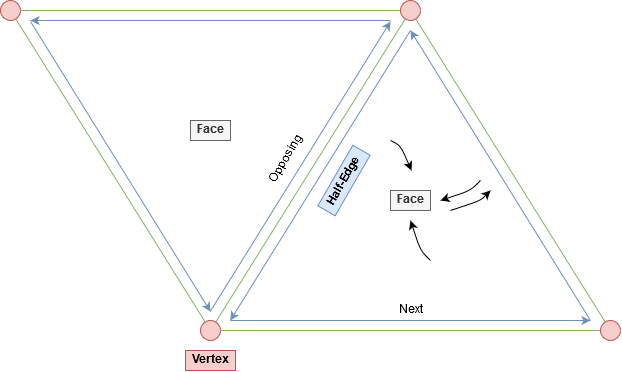
\includegraphics[width=0.7\linewidth]{Images/half-edge-mesh}
	\caption[Half-Edge-Mesh Schematik]{Die Elemente eines Half-Edge-Mesh.}
	\label{fig:half-edge-mesh}
\end{figure}

\subsection{Klassenstruktur}
Aus den beschriebenen Elementen einer Half-Edge-Netzstruktur ergibt sich das in Abbildung \ref{fig:classdiagramhalfedgemesh} gezeigte Klassendiagramm. Der grundlegende Aufbau der einzelnen Klassen basiert dabei auf dem Plankton-Mesh \cite{Meshmash2017}. Jede Komponente besitzt eine eigene Listenklasse. Allerdings besitzen die einzelnen Komponenten im Plankton-Mesh keine direkte Referenz auf die benachbarten Komponenten, sondern einen Verweis auf den Index der Elemente in der jeweiligen Liste. So hat eine Half-Edge keine weitere Half-Edge als ,,Next'', sondern ein den jeweiligen Index der n\"achsten Kante.

\subsection{Die Vertex, HalfEdge und Face Klassen}
Die Klassen \textit{Vertex, HalfEdge} und \textit{Face} sind die Datenmodelle der oben beschriebenen Komponenten. Die Vertex-Klasse besitzt einen \textit{Vector3} Point, der die Position im Raum darstellt, eine \textit{HalfEdge}, die von diesem Punkt aus geht (Im Gegensatz zu \cite{Meshmash2017} wird hier eine Referenz gespeichert.) und der Index des Punktes, um die Arbeit mit dem Unity-Mesh zu erleichtern. Zudem kann ein \textit{PositionChangedEvent} abonniert werden, um Positions\"anderungen im Unity-Mesh direkt zu zeigen.
\\
Eine Half-Edge besitzt die oben erw\"ahnten Eingenschaften: den Punkt von dem sie ausgeht, die anliegende Face, die gegen\"uberliegende und n\"achste HalfEdge sowie den Index der HalfEdge. Wie auch der Index der Vertices, ist dieser Index f\"ur das Unity-Mesh wichtig.
\\
Die Face-Klasse besitzt nur eine Referenz auf eine anliegende HalfEdge.

\subsection{Listenklassen}
Objekte der Klassen \textit{Vertex, HalfEdge, Face} werden jeweils in einer Listenklasse gespeichert. Die Klassen \textit{VertexList, HalfEdgeList, FaceList} implementieren das \textit{IEnumerable}-Interface, um die Iteration \"uber die Elemente zu vereinfachen. Zudem beinhalten diese Klassen die Kernlogiken f\"ur die Komponenten. VertexList bietet die M\"oglichkeit, einen neuen Vertex hinzuzuf\"ugen oder einen zu entfernen, die HalfEdgeList verf\"ugt \"uber eine  \textit{CreateHalfEdge}-Methode, die wie folgt eine HalfEdge anlegt:

\begin{lstlisting}

public HalfEdge CreateHalfEdge(Vertex vertex, Face face, HalfEdge next)
{
	var halfEdge = new HalfEdge(vertex, face, next, Count);
	vertex.HalfEdge = halfEdge;
	_halfEdges.Add(halfEdge);
	return halfEdge;
}

\end{lstlisting}

Und auch die FaceList besitzt eine Create-Methode, um eine Fl\"ache korrekt anlegen zu k\"onnen. Dabei wird die Referenz der Face auf die HalfEdge gesetzt und umgekehrt. Eine Weitere wichtige Methode ist die \textit{GetFaceCirculator}-Methode, die eine Liste aller HalfEdges, die an einer gegebenen Face anliegen, zur\"uck gibt.

\begin{figure}[h]
	\centering
	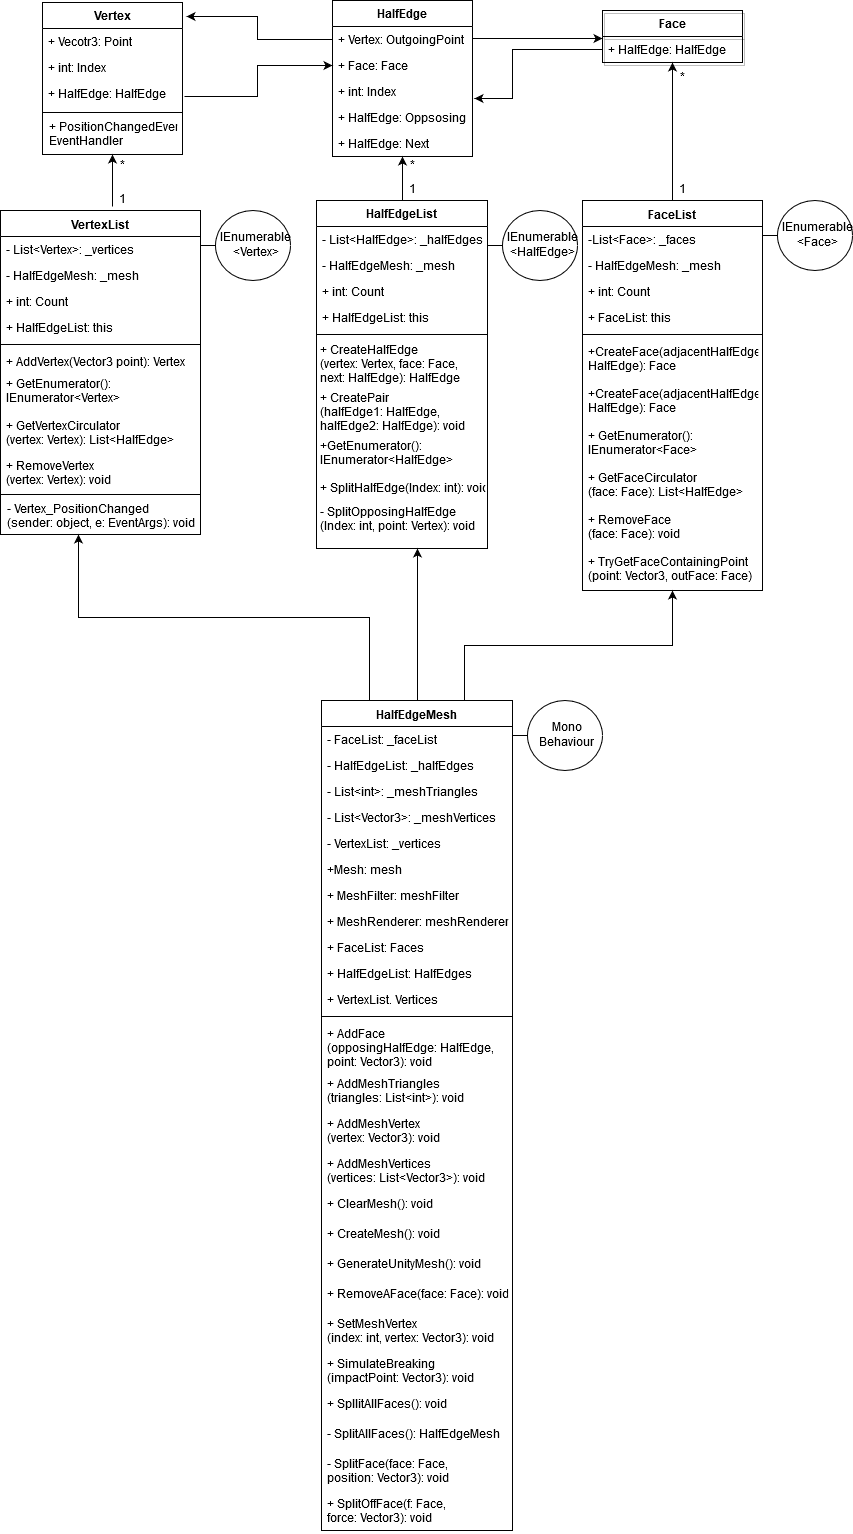
\includegraphics[width=0.7\linewidth]{Images/ClassDiagramHalfEdgeMesh}
	\caption[HalfEdgeMeshUMLDiagramm]{UML-Klassendiagramm des Half-Edge-Mesh Projekts}
	\label{fig:classdiagramhalfedgemesh}
\end{figure}


\section{Implementierung des Half-Edge-Mesh}
Die Oben genannten Listenklassen werden von der \textit{HalfEdgeMesh}-Klasse verwendet, um aus der beschriebenen Half-Edge-Datenstruktur ein von Unity renderbares Mesh zu erstellen. 